
\chapter{Approach}
\label{cha:approach}

The central idea of the thesis is based on the assumption that humans do their activities in the context of time. Humans follow a certain routine in their lifestyles and time is one de-facto latent element in determination of these routines. Most of the activities in ones daily life can be associated with the time of the day. Thus time is a prominent factor while learning human behaviours and preferences. All the models developed in this thesis try to learn human behaviours and preferences based on time as factor. 

\section{Problem Formulation}
In this thesis we use Bayesian models for representing the learned knowledge about human behaviour and preferences. We formulate the problem as getting an accurate probability density of possible locations given the previous observed locations. Given the corresponding observations of $D_{o_i}$, the probability distribution over the locations of $o_i$ at time $T$ is governed by the following formula 

    \begin{equation} \label{eq:1}
	    P(l_i | t_i, D_{o_i})
    \end{equation}

   Various temporal information related to periodic patterns can be implied by $T$, to indicate the location distribution. Such as specific hours of the day (11:00 pm), a day of the week(Friday), or a month of the year(February). We use the \textbf{temporal state} to represent such information and introduce $r(t)$ to denote temporal state extracted from time $T$,.  Dependency on the type of the temporal state $r(t)$ can be a different function. For example,if $r(t)$ denotes temporal state in terms of hours of the day then $r(t) \in {0,1 ... , 23}$, if $r(t)$ denotes temporal state in terms of day of the week, then $r(t) \in {0,1, .. 6}$ . Without loss of generality, we use $r(t)$ to denote a type of temporal state in the following description, Equation \ref{eq:1} is reformulated as 
    
    \begin{equation}
	    P( l_i | r(t), D_{o_i})
    \end{equation}
    
    Applying Bayes Rule
    
    \begin{equation}\label{eq:3}
	P( l_i | r(t), D_{o_i}) \propto P(r(t) | l_i, D_{o_i})  P(l_i | D_{o_i})
    \end{equation}
    Where:
    \begin{itemize}[label=]
    \item $P(r(t) | l_i, D_{o_i})$ : Temporal context 
    \item $P(l_i | D_{o_i})$ : Spatial context
    \end{itemize}
    
     The spatial context $P(l_i | D_{o_i})$ indicates the location distribution of object or person $o_i$ given the previous observed location $D_{o_i}$ . The temporal context $P(r(t) | l_i, D_{o_i})$ represents the temporal state distribution of object $o_i$, being observed at location $l_i$ with corresponding $D_{o_i}$
    


\begin{tabular}{cp{8cm}}
    \hline
	Symbol & Meaning\\
	\hline
	O & Set of all objects or persons\\
	$o_i$ & Single object from the set $O$, $o_i \in O$ \\
	$L$ & Set of all locations\\
	$l_i$ & Single location from the set $L$. $l_i\in L$\\
    $T$ & Time interval\\
    \hline
	$<o_i,l_i,t_i>$ & object $o_i$ was located at location $l_i$ at time $t_i$\\
	$D$ & Collection of all objects all observed locations\\
	$D_{o_i}$ & Previous observed locations of $o_i$\\ 
    \hline
     $P(r(t) | l_i, D_{o_i})$ &  Temporal context representing the temporal state distribution of $o_i$ at location $l_i$ given previous observations $D_i$\\
     $P(l_i | D_{o_i})$ & Spatial context representing the location distribution of object $o_i$ given the previous observations $D_{o_i}$\\
    \hline
\end{tabular}
% section Problem formulati (end)

\section{Model Implementation}

In this thesis, we use probabilistic approach to knowledge acquisitions, which models learning and reasoning as inference in complex probabilistic models. In particular, we examine how robots can quantitatively  develop knowledge from information,  modelled using  functional probabilistic programming languages. 


\section{DIKW pyramid}
\todo[inline]{TODD}

\section{Architecture}
\todo[inline]{TODO
Robot uses records it sensors values ,
Robot uses the sensors readings and converts to information ,
the information is stored in robot memory. 
On regular basis or on trigger the the knowledge generation software is trigger which generates the knowledge and adds back to the robot memory 

}
\label{cha:}
\begin{figure}[htp]
\centering
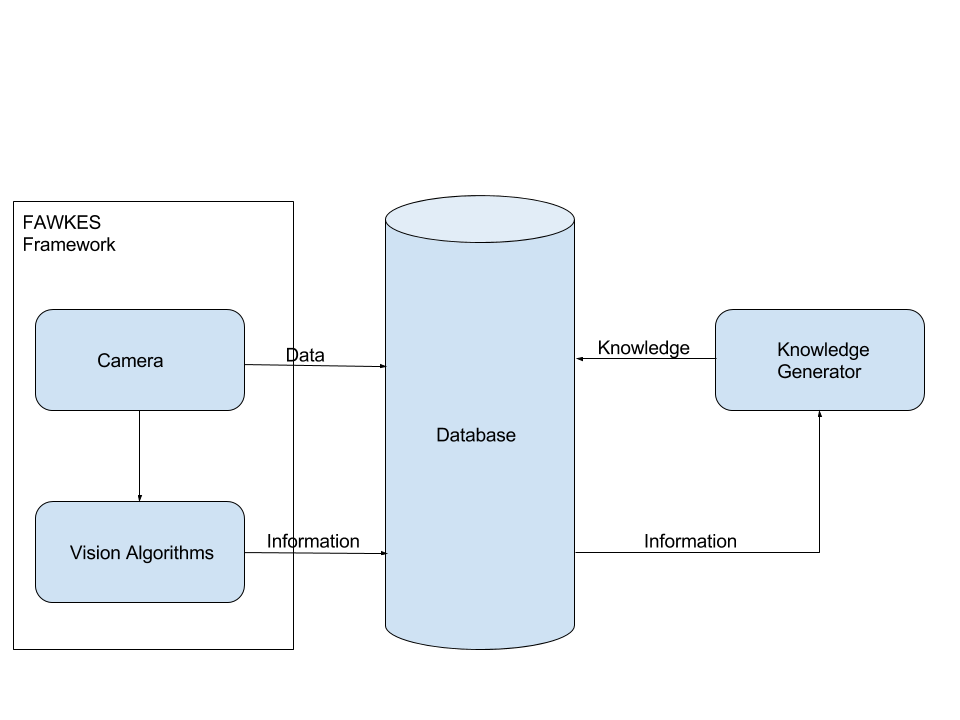
\includegraphics[width=\textwidth]{images/integration.png}
\caption{Integration with the robot memory}
\label{}
\end{figure}


\section{Notation and terminology}
Throughout the thesis, we are referring to entities such as ``locations," ``hours," and ``observations".
This helps to guide intuition and maintain continuity of thoughts as we guide through related problems involving collections of data.
Formally we define the following terms:
\begin{itemize}
	\item A \emph{location} is the basic unit of the discrete data, defined to be an item from a set of locations. These locations can be rooms of the home or different compartments of the kitchen. 
	\item An \emph{period} is a sequence of $N$ locations denoted by $\textbf{p} = {x_1;x_2;:::;x_N}$. These represents the locations observed in a particular period of time.
	\item A \emph{observations} is a collection of $T$ periods denoted by $ D = {p_1;p_2;:::;p_T}$. These represents the complete data collected by the robot.
\end{itemize}


We also use the entities such as ``data," ``information," and ``knowledge" throughout the thesis. These can be define as:
\begin{itemize}
	\item A \emph{data} corresponds to sensor output. All the output of the sensors recorded by the robot is a data. For example RGB image from a camera, depth points from depth sensors etc.
	\item A \emph{information} corresponds to output of algorithms which process on the above data. For example vision algorithms process RGB images data to extract information of objects or persons in the image.
	\item A \emph{knowledge} corresponds to output of algorithms which process on the above information. For example vision algorithms can process detected object information in consecutive RGB frames to extract knowledge that the object was moving.
\end{itemize}

% section  Things to study (end)